%!TEX root = ../main/main.tex
\section{Runtime View} % (fold)
\label{sec:runtime_view}
\subsection{Server View} % (fold)
\label{sub:server_view}

% subsection server_view (end)
In this section we focus on the \emph{Runtime View} of the system.\\
While the system is up and running, the \emph{Server} receives many \emph{HTTP} requests from different clients that are handled by a \emph{Load Balancing} component that distributes the calls uniformly to every real machine.\\
Every request from the users are registered by the server and saved in the \emph{MySQL} database.\\
From the \emph{internal} point of view of the \emph{Back-End} application, request are at first parsed by the \emph{Request Manager} and the dispatched to Java object that is in charge of computing the result of that request. Three diagrams are provided to better exemplify the flow of events.\\
\subsection{Client View} % (fold)
\label{sub:client_view}

% subsection client_view (end)
From the client point of view, when a \emph{User} or a \emph{Taxi Driver} open his app, the client starts a first \emph{"handshake"} to check for basic authentication data and if it's successful, the client can proceed with requests.\\
The flow of a request start from a \emph{UI} component (like a \emph{button}) and is finally handled by the class that implements the \emph{HTTP} interface.
% section runtime_view (end)


\newpage
\vfill
\begin{figure}[h!t]
\caption{Modify Personal Data}
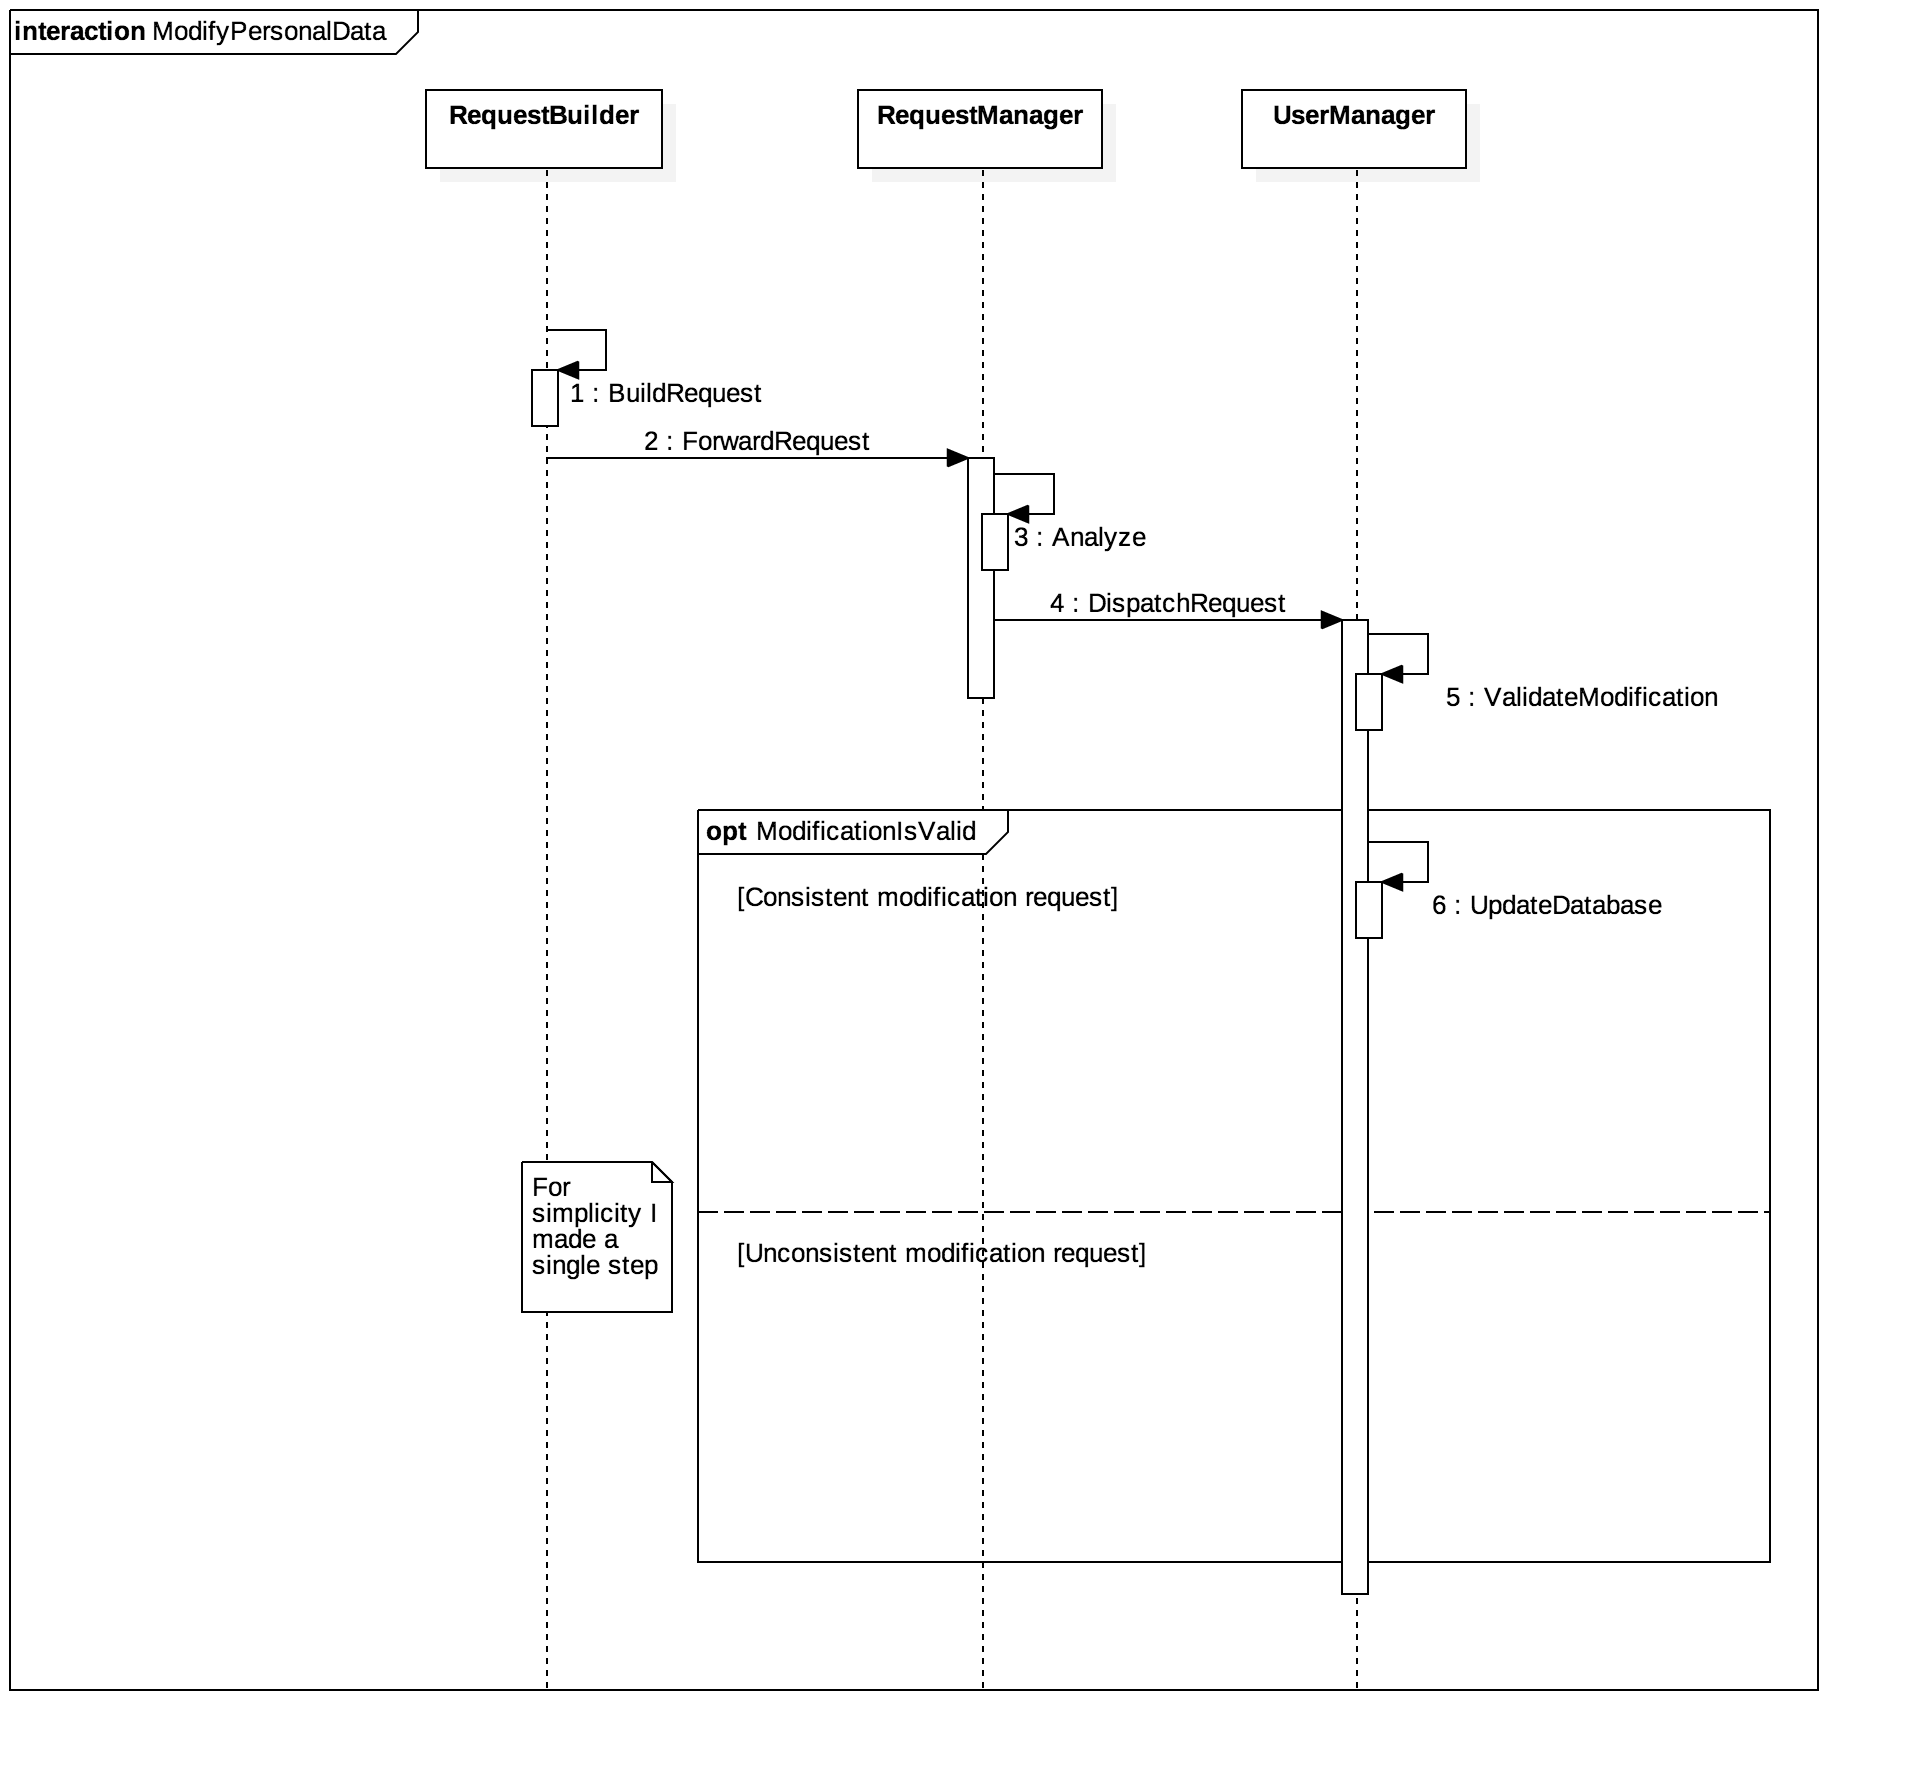
\includegraphics[width=\textwidth]{diagram/png/modify}
\centering
\end{figure}
\vfill
\clearpage

\newpage
\vfill
\begin{figure}[h!t]
\caption{Taxi Request}
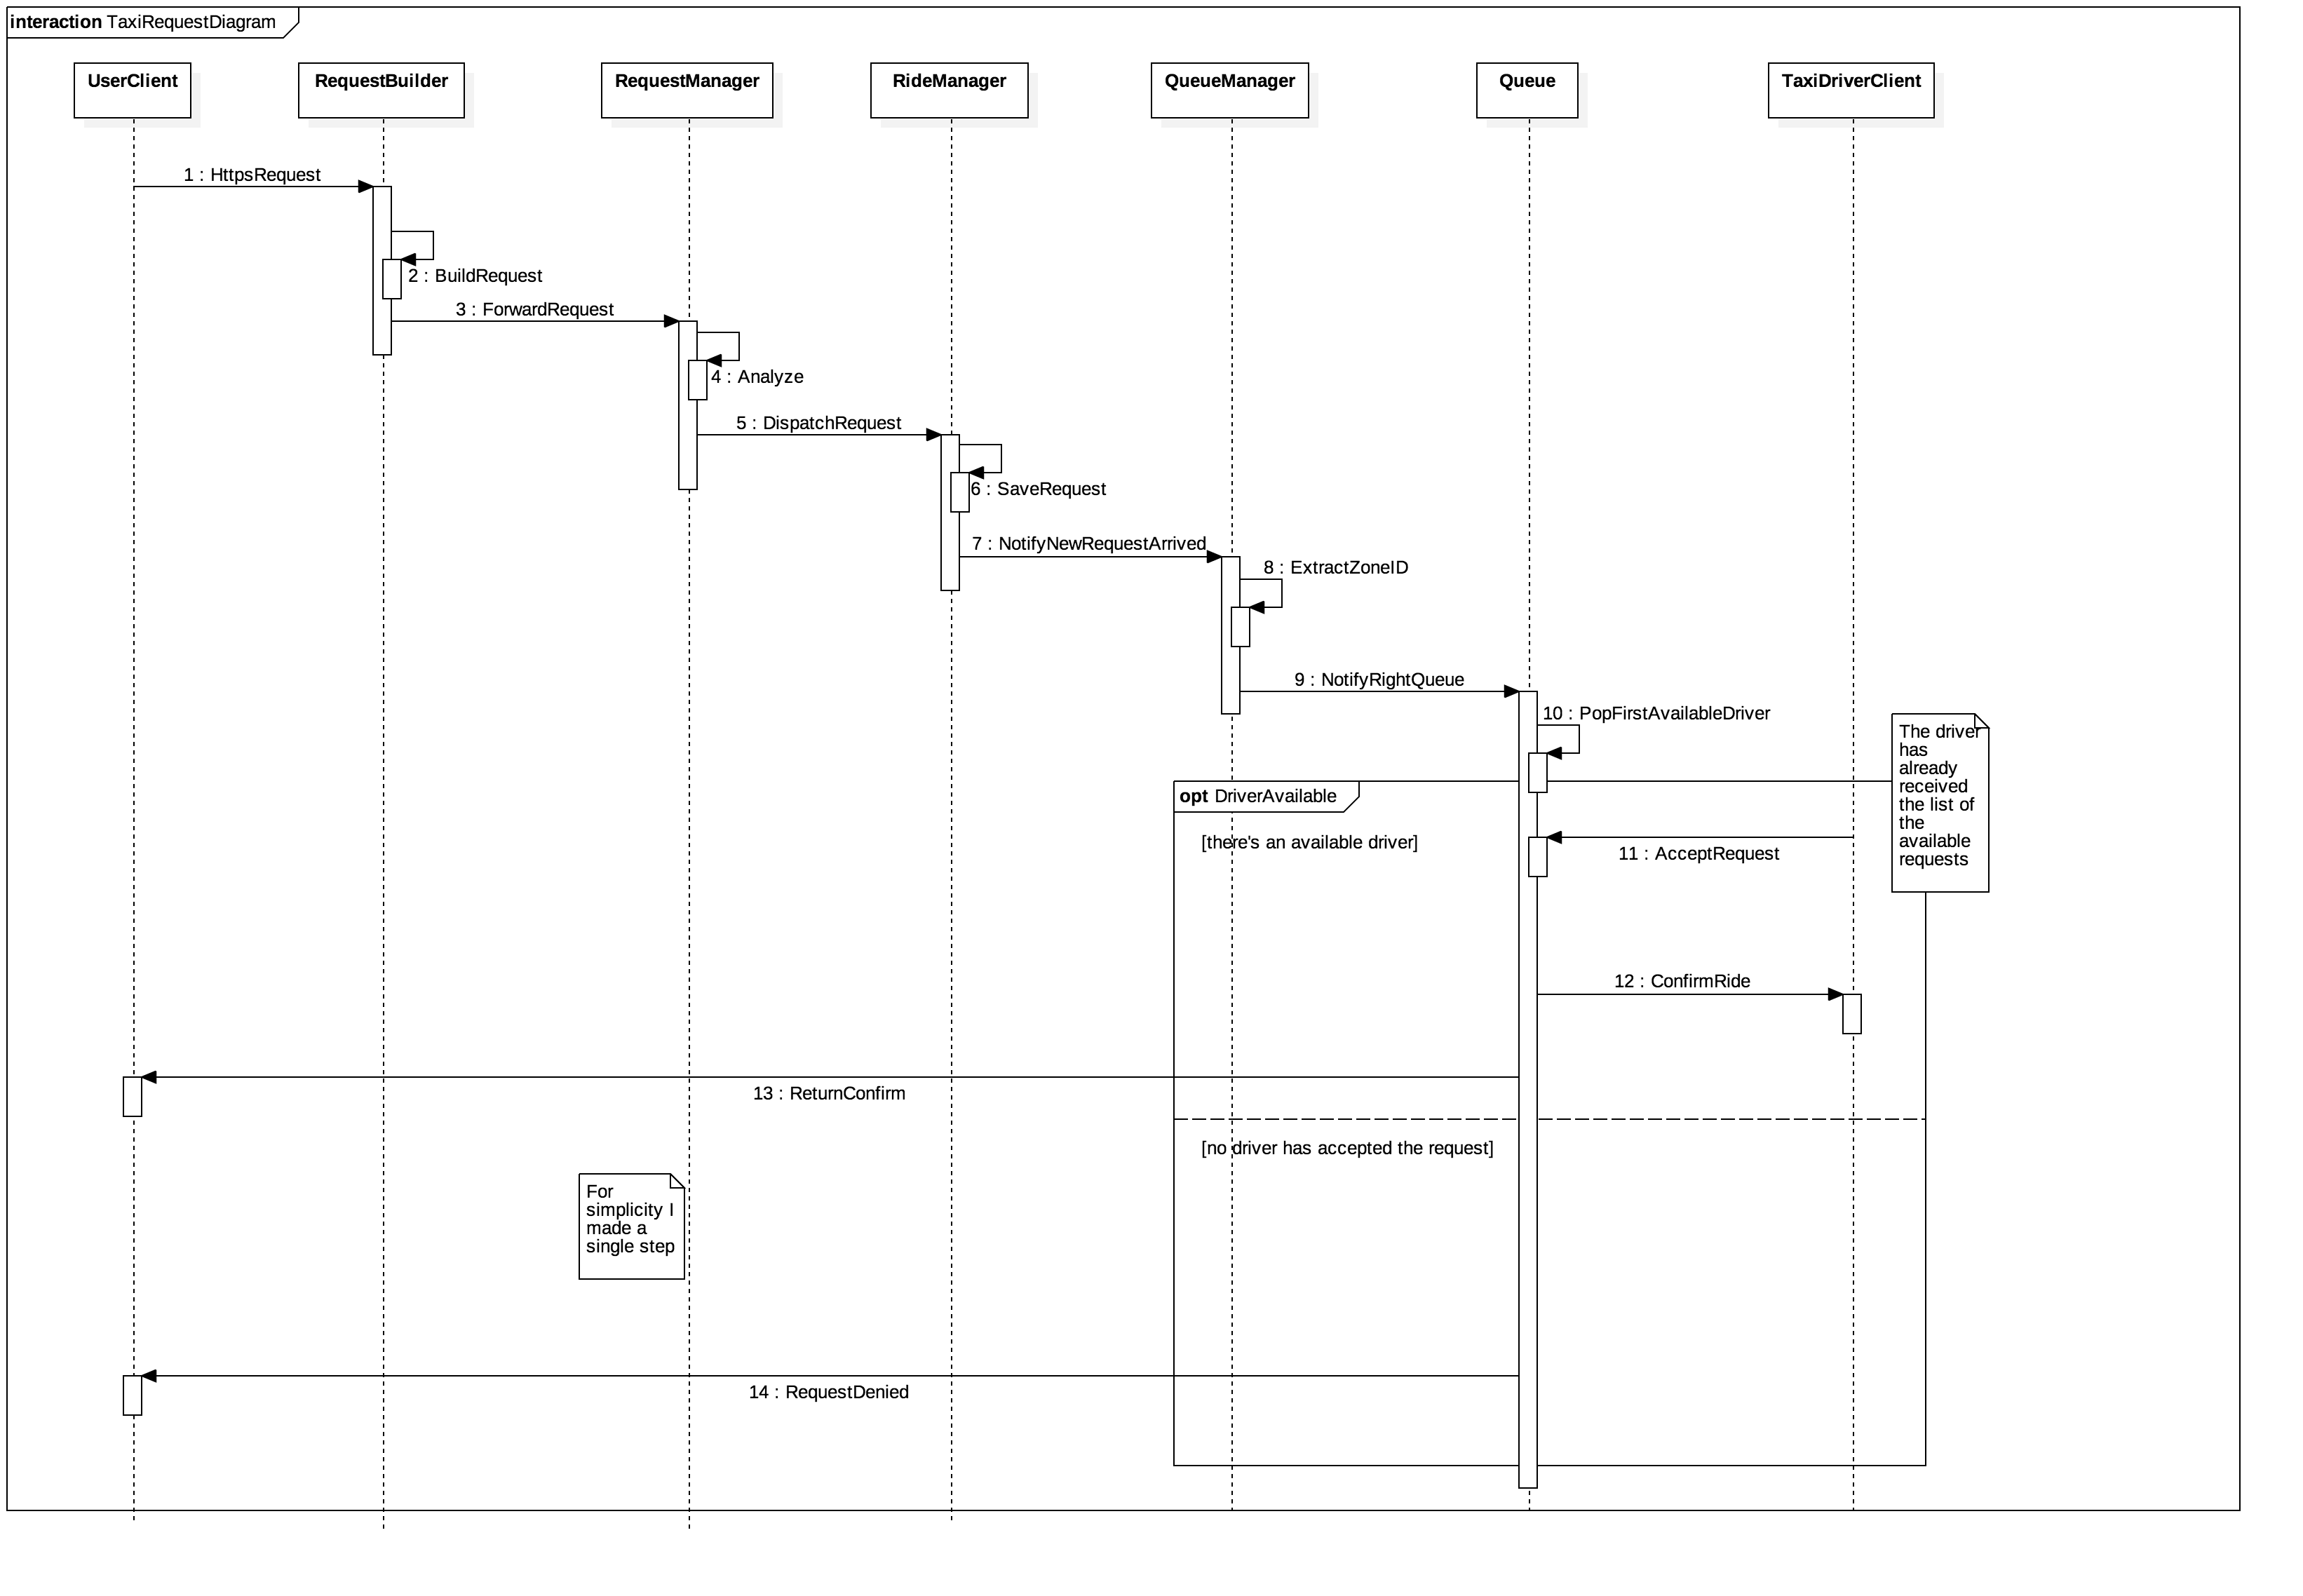
\includegraphics[width=\textwidth]{diagram/png/request}
\centering
\end{figure}
\vfill
\clearpage

\newpage
\vfill
\begin{figure}[h!t]
\caption{Update Taxi Position}
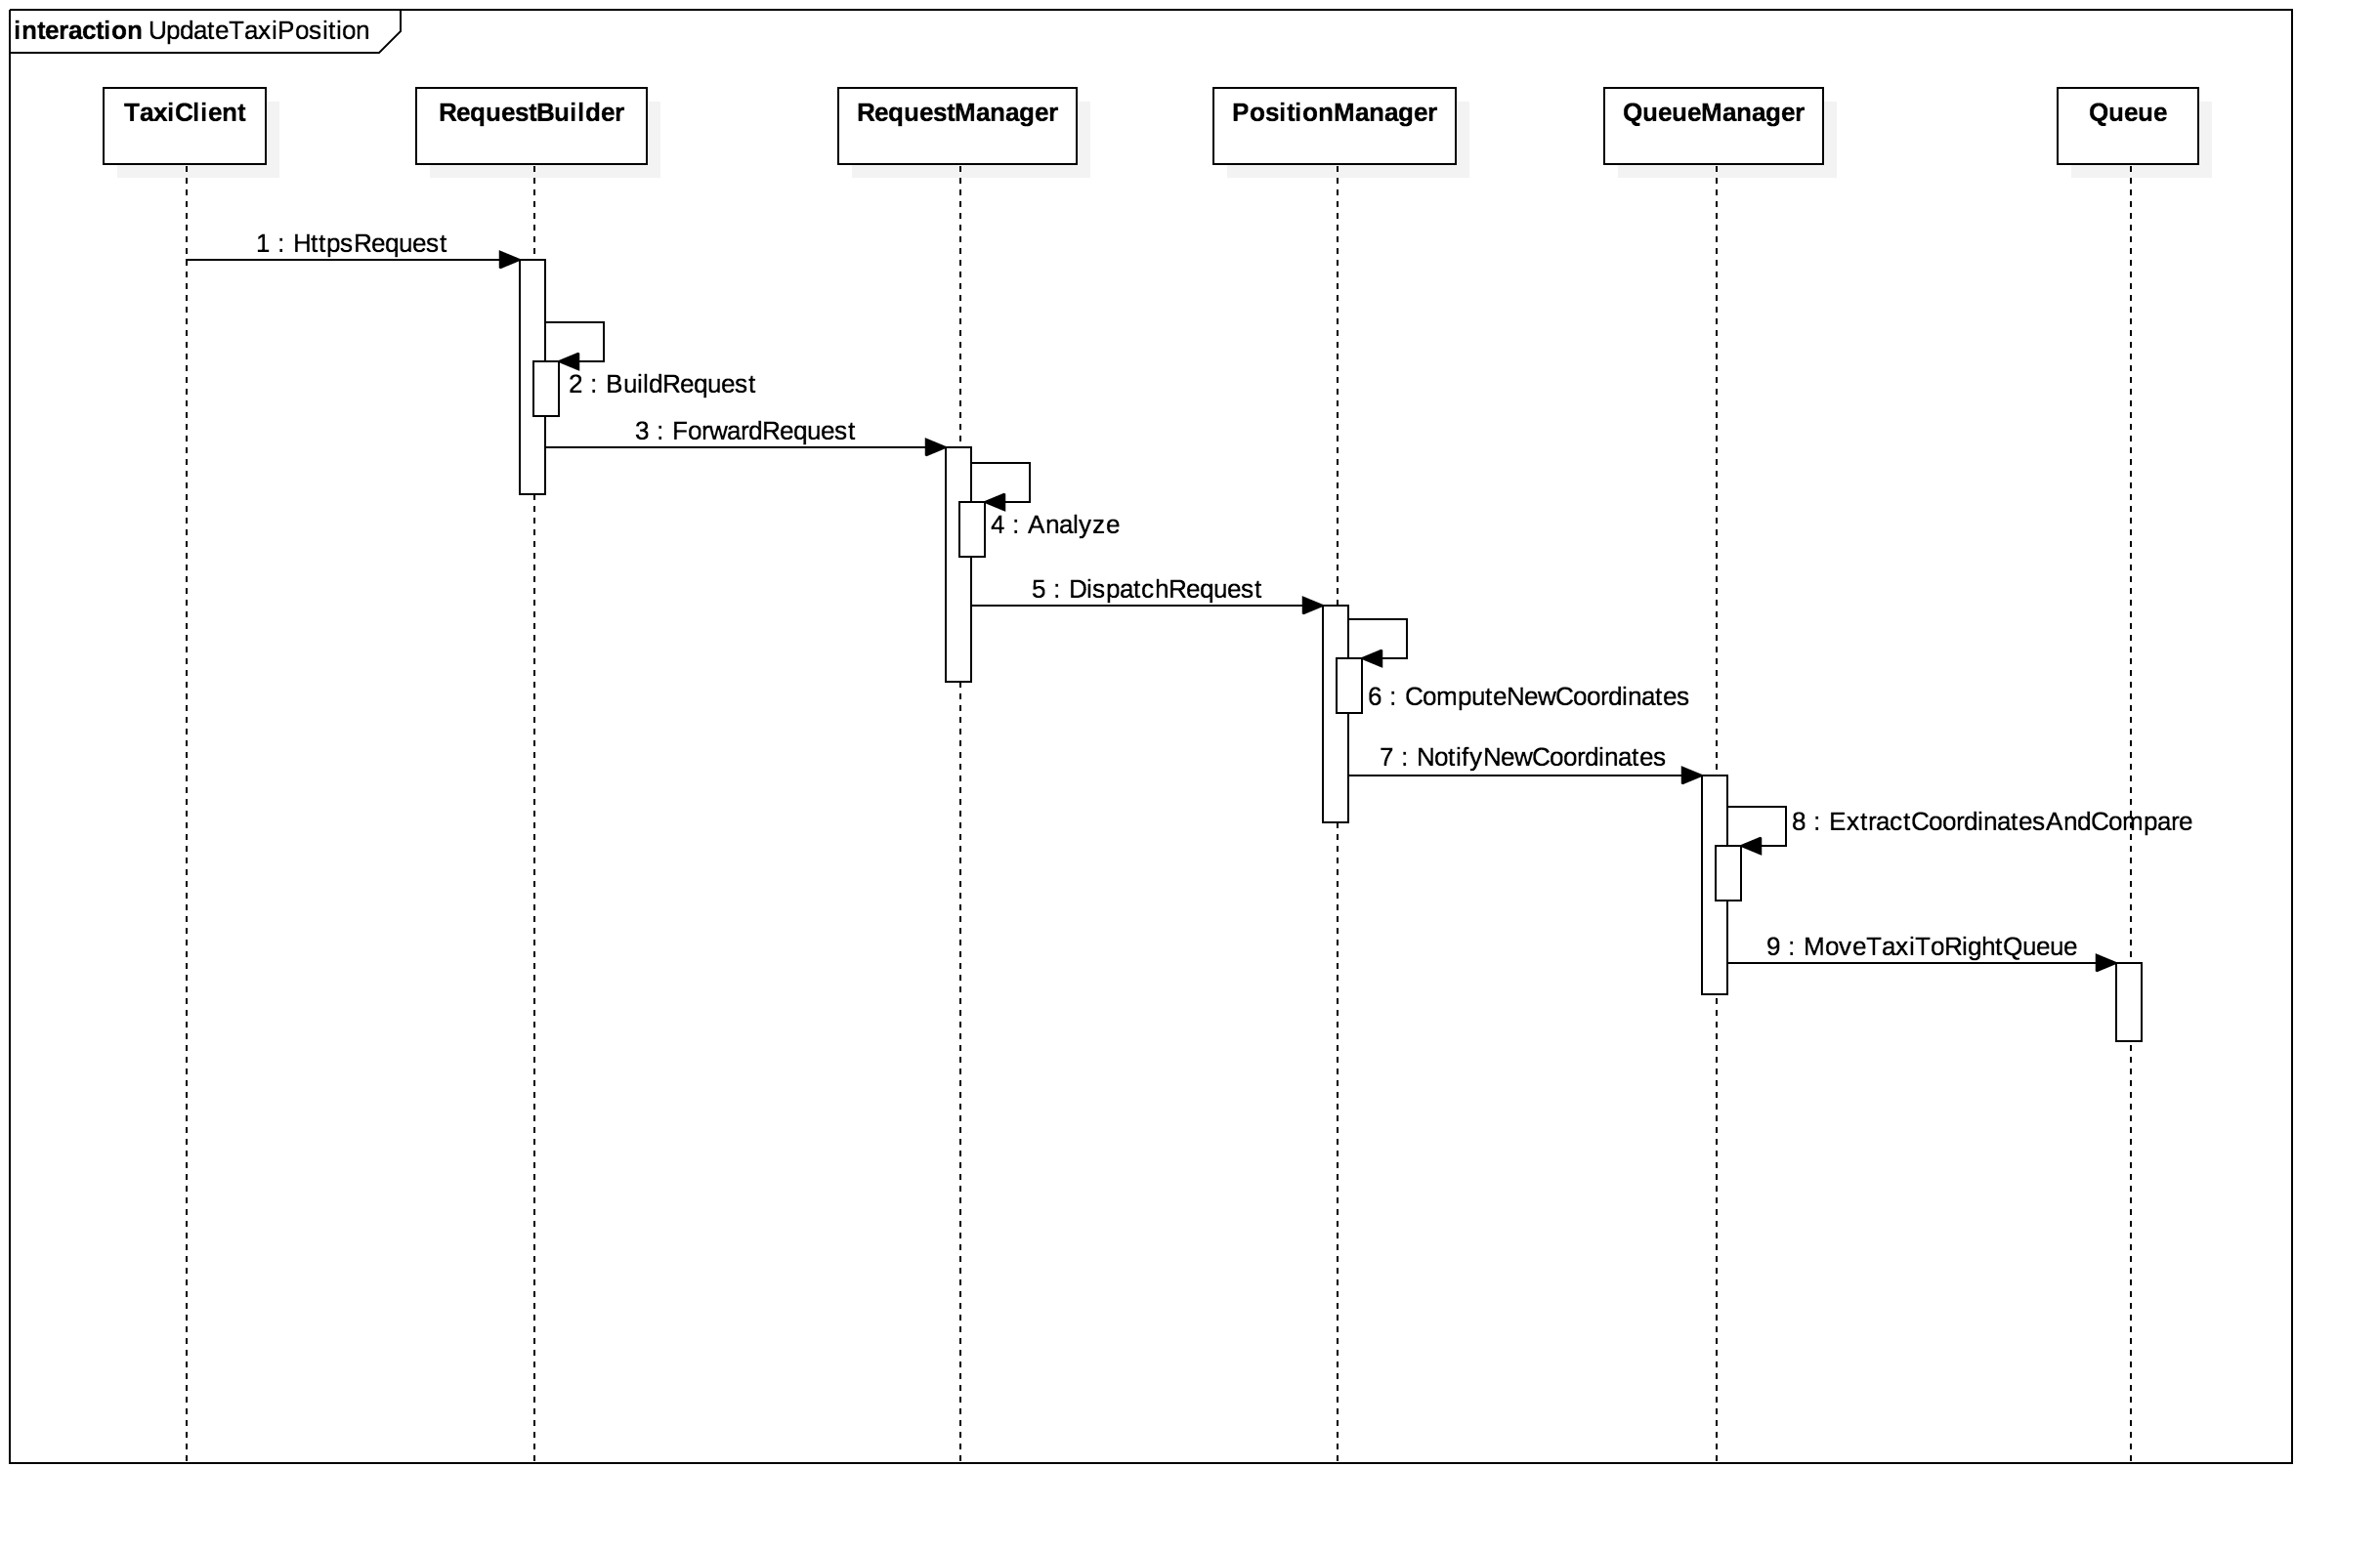
\includegraphics[width=\textwidth]{diagram/png/updateTaxi}
\centering
\end{figure}
\vfill
\clearpage



